\documentclass[oribibl]{llncs2e/llncs}
\usepackage{geometry}                % See geometry.pdf to learn the layout options. There are lots.
\geometry{letterpaper}                   % ... or a4paper or a5paper or ... 
%\geometry{landscape}                % Activate for for rotated page geometry
%\usepackage[parfill]{parskip}    % Activate to begin paragraphs with an empty line rather than an indent
\usepackage{amssymb,amsmath}
\usepackage{graphicx}
\usepackage{amssymb}
\usepackage{epstopdf}
\DeclareGraphicsRule{.tif}{png}{.png}{`convert #1 `dirname #1`/`basename #1 .tif`.png}

\graphicspath{{WarpTask/figures/}{Res/figures/}} %do not forget the / at the end
%\include{{llncs2e}}
\title{Very Large Integers  and polynomial inner product}
\author{Timoth\'ee Ewart\inst{1}\thanks{Acknowledgments: Maxim Milakov, Peter Messmer  - NVIDIA, and  Williams Sawyer, Gilles Fourestey - CSCS}  , Andreas Hehn$^2$, Matthias Troyer\inst{2} and Thierry Giamarchi\inst{1}}

\institute{Universit\'e de Gen\`eve, \email{timothee.ewart@gmail.com}  \and Eidgen\"ossische Technische Hochschule Z\"urich }

%\date{}                                           % Activate to display a given date or no dater
\begin{document}
\maketitle
%\section{}
%\subsection{}
%\vspace{-0.65cm}
\begin{abstract}
The main purpose of the  Very Large Integer (VLI/C++) library is to perform large integer arithmetic and  inner product of polynomials. Based on meta-programming of assembly,
and  hybrid (CPU/GPU) mode, it performs inner product of dense and triangular polynomials  of 1 to 4 variables  up to order 14. The coefficients are represented  by large integers of 128 to 256 bits. 
In this paper, we remember the basics of the inner product with polynomials, and  we present the implementation of the library in assembly. Then, we focus on the GPU implementation of the inner product.  All our algorithms are based on brute force attacks, because the problem is too small for a FFT approach to be valuable. We save a factor up to 10 on CPU and 60 on GPU compared to a GMP solution.
We get 67 \% of the peak performance of the GPU.
\end{abstract}
\section{Introduction}
 A few libraries like  LINBOX or NTL  provide high performance in polynomial solvers.
These libraries are  connected with GMP\footnote{GMP is the standard library for long arithmetic, gmplib.org} when needed. 
The introduction of hardware accelerators in HPC a few years ago, and more recently of GPU  by NVIDIA, introduce a revolution in the programming models. 
It is therefore necessary  to adapt the libraries to these new hardwares.  The most famous example on this transition is the famous blas/lapack libraries to MAGMA. 
Polynomials libraries, however  did not yet  make the transition to GPU.
During the last few years, the polynomial multiplication was successfully implement to this new hardware
\cite{Govindaraju2008, Emeliyanenko:2009, Moreno2010}. All these works focus on large polynomials,
 using a FFT approach. 

In the present work, we are focusing on the inner product of dense and triangular multivariable polynomials.  The coefficients of the polynomials are large integers. 
We preferred to develop a long integer library  rather than utilizing GMP, because GMP is a dynamic library.
Moreover, we want a library natively compatible with GPU to allow hybrid calculation. GPU imposes contiguous memory which is impossible with a GMP approach.
Thus, we propose a static library based on contiguous memory where the exact assembly kernels are generated by meta-programming during the compilation for CPU and GPU.
We do not waste time in the dynamic memory allocation, and let the compiler optimize deeply the library for both architectures.

\section{Polynomial and inner product definitions}

The library performs the inner product of vectors of polynomials from one to four variables, where polynomials are defined like (four variables) :
\begin{eqnarray}
P_a(x,y,z,w) & = & \sum_{i=0}^n \sum_{j=0}^n  \sum_{k=0}^n \sum_{l=0}^n  a_{ijkl} x^i y^j z^k w^l , \,\,\,\,\,\, \text{or} \\
                   & = & \sum_{i=0}^n \sum_{j=0}^{(n-i)} \sum_{k=0}^{(n-i-j)} \sum_{l=0}^{(n-i-j-k)}  a_{ijkl} x^i y^j z^k w^l  .
\end{eqnarray}
where  $x,\,y,\,z$ and $w$ are the variables,  $i,\,j,\,k$ and $l$  the indices, $a$  the coefficients, and $n$ the order of the polynomial.
The polynomials of the form  (1) and (2) are named dense and triangular respectively. Consider now two vectors of polynomials of the  same type with $m$ 
entries  $\boldsymbol{v}_1<P_a>$ and  $\boldsymbol{v}_2<P_b>$. The inner product  consists in the product 
of every entries  associated with a global reduction. 
 \begin{eqnarray}
 P_c = \sum_i^m \boldsymbol{v}_{1_i}<P_a>  \times  \boldsymbol{v}_{2_i}<P_b> \label{poly1} \label{InnerProduct}
\end{eqnarray}
where $\times$ indicates the multiplication between two polynomials. The multiplications use basic rules of polynomials multiplication. 
A final coefficient may be the sum of several coefficients (named contributions), resulting from the sum of several multiplications. These coefficients are the cross terms. 
The cross terms are not a problem for the CPU version, as a polynomial multiplication is done by a single thread, but they are the bottleneck for the GPU version.
The number of coefficient for a dense and triangular polynomial is given by $(n+1)^{\kappa}$ and  $(\kappa+n-1)! / ( (\kappa-1)! n! )$ respectively, where $\kappa$ is the number of variables. 

In terms of  programming and parallelization, at least for the CPU version, the previous equations can be reduced to independent loops with a final reduction.
The CPU parallelization has been done with OpenMP. The OpenMP threads calculate several  polynomial multiplications and make a local reduction. At the end, a final reduction is performed  by the main thread.
 % \footnote{In OpenMP reduction for class is not supported}. Results showed a perfect scalability of the OpenMP code. 

\section{VLI  CPU library}

The coefficients of the polynomials are represented by a large integer named VLI number.  A VLI number is characterized by a size in bits; the size is a  template parameter, which
varies from 128 to 512 bits.  Its implementation is static, contrary to GMP. 
Inside the memory, the VLI numbers are  contiguous. The data type container is a 64 bits unsigned integer array.

The basic operations supported by VLI are the four basic operations: $+,-,\times, /$, extended multiplications and bit shift. The library allows  operations between operands of the same type, and with basic  integer. For performance reasons, we have a specific solver for every operation except  the division. All the algorithms and operations are based on the elementary  methods that we learn 
in our the childhood but the realizations has been done in assembly,
because the assembly instructions facilitate the implementation and boost the performances.

\subsection{Assembly}

We applied algorithms based on childhood  experience for large arithmetic. These methods necessitate carry\footnote{ The carry bit is a bit of the register of status, as the overflow bit, 
it informs  the overflow of an operation, but it can be re-used to propagate the carry. } for addition/subtraction and an extended multiplication for the multiplication.
Although the hardware supports them, we can not access  these features by the C++ language. The only possibility is the assembly language.

In assembly, these operations  are supported by the pair of mnemonics; \texttt{addq/adcq} for the addition; \texttt{sbbq/subq} for the subtraction, and \texttt{mul} for the extended multiplication.   
Combining these mnemonics, we reproduce easily long arithmetic algorithm, as described into the famous  ASM book of \cite{Hyde:2003:AAL:861534}. 

We coded the assembly using the GNU inline assembly which consists of strings between ASM tags.
Generating by hand all these  assembly strings (kernels)  can be painful and a source of error\footnote{The library has near 10000 lines of assembly cumulated between x86-64, Power64, and PTX} 
We designed a generator of assembly. It creates all versions of a kernel during the compilation.   
It is built on the preprocessor with the boost preprocessor package. We can thus create and manipulate the ASM strings during the precompilation, 
and generate a specifically tuned kernel for every large integer. We give a small example of a long addition with the generator into the table \ref{ASMGENERATOR}.

 \begin{table}[h] 
	\begin{center}
	 	\begin{tabular}{l l}
                           \hline 
                           \textbf{Assembly generator}      \hspace{8.5 cm}  ASM  x86-64 \\ \hline
                           \begin{tabular}{l l l l } 
                               \tiny{1:} & begin asm(\texttt{"}     &  $\vartriangleright$ Start ASM string & asm(\texttt{"} \\
                               \tiny{2:} &  \textbf{boost  repeat} over n  &$\vartriangleright$  Start the repetition over n from 0 to n-1 &   \\
                               \tiny{3:} &   \hspace{0.2 cm}  boost  if(n = 0) &  $\vartriangleright$   if n = 0 &  \hspace{0.2 cm}  \texttt{"}\texttt{addq} 0x0(rsi), rax\texttt{"}\\    
                               \tiny{4:} &   \hspace{0.4 cm}  boost stringize(\texttt{addq}  $r_i$, $r_j$)  &$\vartriangleright$   Become \texttt{"addq} \dots &  \hspace{0.2 cm}    \texttt{"}\texttt{adcq}  0x8(rsi), rax\texttt{"}\\    
                               \tiny{5:} &   \hspace{0.2 cm}  boost  else  & $\vartriangleright$   if n != 0 &  \hspace{0.2 cm}  \texttt{"}\texttt{adcq}  0x10(rsi), rax\texttt{"} \\ 
                               \tiny{6:} &   \hspace{0.4 cm}  boost stringize(\texttt{adcq}  $r_i$, $r_j$)  &$\vartriangleright$   Become \texttt{"adcq} \dots &  \hspace{0.2 cm}   \texttt{"}\texttt{adcq}  0x18(rsi), rax\texttt{"}\\     
                               \tiny{7:} &  \textbf{end boost repeat} &  &   \\                            
                               \tiny{8:} &  \texttt{"})  &  $\vartriangleright$ end ASM string & \texttt{"})\\
                          \end{tabular} &  \\ \hline
		 \end{tabular} 
		 \caption{Basic example of the ASM generator for a long addition (n=4), the preprocessor with the boost preprocessor macros generate the effective string for the ASM block. ASM \texttt{move} are not included, as the correct use of the registers. It exceeds  the purpose of the present document \label{ASMGENERATOR}.  }
	\end{center}
\end{table} 

The x86-64 architecture allows 16 registers (32 for power). As much as possible, in the solver, we conserve the data in the registers in order to reduce memory read/writes to the  minimum.
 Additional optimizations have been done like full unrolling or assembly tips. We  supported  x86-64, Power64 and PTX (GPU) assembly.
 PTX does not support carry bit for 64 bits integer, but only for 32 bits integer\footnote{Introduced since CUDA 4.2}.  
It allows multiplication-addition of 32 bits integers  with carry bit support \cite{CUDAasm}. 
Work in 32 bits mode imposes twice as much operations for the additions/subtractions, and one order of magnitude more for the multiplications. 

\subsection{Memory layout and SIMD implementation}

There exists at least two data layouts for this problem: the array of structure (AoS) and structure of array (SoA). Both have  advantages and disadvantages. In our problem the AoS consists in saving the data in this order : VLI - series of VLI (polynomial coefficient)- series of polynomials (the vector). The SoA structure interleaves the coefficients of the VLI and the polynomials.

%\begin{figure}
%\begin{minipage}{0.50\linewidth}
%\begin{eqnarray}
%\tiny{
% \underbrace{
% \underbrace{ \underbrace{a^0_{00} | a^1_{00} | a^2_{00}}_{VLI, a_{00} } || \underbrace{a^0_{10} | a^1_{10} | a^2_{10}}_{VLI, a_{10}} ||   \dots  }_{1^{st} \textrm{polynomial}} 
%      |||    \underbrace{ \underbrace{b^0_{00} | a^1_{00} | b^2_{00}}_{VLI, b_{00} } || \underbrace{b^0_{10} | b^1_{10} | b^2_{10}}_{VLI, b_{10}} ||   \dots  }_{2^{nd} \textrm{polynomial} } }_{\textrm{Vector of polynomials, AoS order}} \nonumber
%}
%\end{eqnarray}
%\end{minipage}
%\begin{minipage}{0.50\linewidth}
%\begin{eqnarray}
%\tiny{
% \underbrace{
% \underbrace{a^0_{00} | a^0_{10} | \dots || a^1_{00} | a^1_{10} | \dots  }_{1st  \textrm{ nested VLI/Polynomial} } |||  \underbrace{b^0_{00} | b^0_{10} | \dots || b^1_{00} | b^1_{10} | \dots  }_{2nd  \textrm{ nested VLI/Polynomial} }
% }_{\textrm{Vector of polynomials, SoA Order}} \nonumber }
%\end{eqnarray}
%\end{minipage}
%\caption{Representation of the AoS Order (left) or SoA Order (right) for a vector of polynomial \label{AOSSOA}}
%\end{figure}

The choice of the memory layout is important. It may facilitate  the usage of the SIMD/AVX instructions. We choose the AoS for the following reasons:
we want to reuse the VLI library in other objects conception code, so we can not interleave the VLI number with the polynomial. 
 Apply SIMD on AoS, for an addition is a non sense because there is no specific instruction to propagate carry between entries of the multimedia register.
The extended multiplication under AVX \texttt{\_\_mm256\_mul\_epu32}  allows only four multiplications of 32 bits, we save a factor two. Nevertheless, on Sandy Bridge, we have 3 ALU, we can not exclude
the execution of several long multiplication in the same time, and we lose the benefice of the SIMD version. Moreover, a large extra work is necessary to prepare the registers and shuffle the data into the registers which is expensive. For our range of operations the extended multiplication varies from 128 to 512 bits, a SIMD version will not be the optimal solution. Though, it has been used with sucess for  integers higher than 1024 bits \cite{SIMD}.

\section{A short introduction to GPU}

A Graphical Portable Unit  is efficient  to address problems which can be expressed as data-parallel computations � the same program 
is executed on many data elements in parallel. Successful usage of GPU in HPC requires a good understanding of their design to reach great performance. A GPU is composed 
of several independent calculation  entities named streaming multiprocessors (SMs typically a tenth), where the SMs run hundreds of threads concurrently (typically 256) by group of 32 (warp).
The GPU programming model imposes to divide the problem into coarse sub-problem that can be solved independently in parallel by blocks of threads,
 and each sub-problem into finer pieces that can be solved cooperatively in parallel by all threads within the block. 
% During the execution, independent blocks will be executed on free SMs, where the program of the block is executed over the threads concurrently way.

In terms of memory, all SMs  share  a large  memory (several GigaBytes) with  low performance; approximatively one hundred cycles for read/write operations.
Inside each SM additional special memories (constant, shared, texture, surface) are available. These memories are characterized by their behavior: they can be read only, shared, cache and more.  
They have still a common characteristics, a very high performance for read/write  operations in a few cycles only.
A good programming practice is to preload data from global memory in shared/texture at once, for subsequent computations.  \label{CUDA_PRACTICE}

Applying the GPU ideology to the polynomial inner product  means that the polynomial multiplications will be executed in parallel on the SMs. Then a global reduction will sum all resulting polynomials. The division into blocks is natural, a block being a single entry of the vector (equation \ref{InnerProduct}). All the difficulties consists in designing a parallel algorithm for the polynomial multiplication and the final reduction.

\subsection{Inner product booster on GPU}

\begin{figure}[t]
\begin{center}
\mbox{
\includegraphics[scale=0.37, angle=-90]{coeffs.eps} 
\includegraphics[scale=0.37, angle=-90]{warp.eps} 
}
\caption{Left: Results coefficients (red line) sorted in reverse order and group by warp. Right: Balance of the tasks over the warps.}
\label{algo_GPU}
\end{center}
\end{figure}

The first idea coming in mind: calculate every single multiplication on an independent GPU thread.  Indeed for a dense polynomial, the number of coefficients can be large and compatible with the number of SMs threads. Nevertheless,  the result coefficients may have several contributions. If the contributions are calculated by several threads, this requires reduction between threads. This solution introduces   synchronizations, and leads to low performance.
The peak performance will be reached if the warps run the same amount of work, and every single thread in a warp is responsible for all contributions to an output coefficient.
In order to achieve this goal, we defined a task object. A task is a set of 32 result coefficients in a specific order. A task tells a  warp how to calculate coefficients (the thread number one of the warp takes the first coefficient of the task and so on). The warps may not have the same number of tasks, as we equilibrate the workload.
We proceed in two  steps: first on CPU, where a preliminary work is done, we prepare all information on the tasks, and then, the calculation on GPU.

For the first step, we create a fictive resulting polynomial  represented by the indices and the contributions. They are sorted by descending order of the number of contributions
and grouped by 32 as a task. These tasks are reordered over the warps to equilibrate the amount of work. An illustration of this algorithm is given on  figure \ref{algo_GPU}. 
The more coefficients the polynomials have, the more uniform the distribution of the tasks over the warps will be, and the more efficient the calculation.
We fix the maximum number of warp to eight (8 warps - 256 threads), as far as possible, we assign at least two tasks per warp.
Thus, depending on  the number of coefficients a warp may calculate one task, whereas another warp may have several tasks to calculate.
 When the determination of the task's list is over,  we transfer  asynchronously the tasks list to the global memory.
This method does not  change the ordering of the data. As for the CPU version, we have an AoS order.
 \begin{table}[t] 
	\begin{center}
	 	\begin{tabular}{l l}
                           \hline 
                           \textbf{Task execution}  Algorithm &  \\ \hline
                           \begin{tabular}{c l l} 
                               \tiny{1:} & VLI tmp   &  $\vartriangleright$ Specific to every thread  \\
                               \tiny{2:} &  \textbf{for} over number of task list size &$\vartriangleright$  Depend on the warp \\
                               \tiny{3:} &  tmp $\,\, \wedge=$ tmp     & $\vartriangleright$ Flush to 0 \\    
                               \tiny{4:} &   VLI ResCoeff &$\vartriangleright$  Thread gets a result coefficient from a task \\
                               \tiny{5:} &  \hspace{0.2 cm}  \textbf{for} over the number of contributions  & $\vartriangleright$ Each thread loops over its coefficients \\
                               \tiny{6:} &  \hspace{0.4 cm}   Indices$_i$ = GetIndices(ResCoeff) &$\vartriangleright$ Determine input indices \\
                               \tiny{7:} &  \hspace{0.4 cm}   tmp + = CoeffPoly$_1$(indices$_1$) $\times$ CoeffPoly$_2$(indices$_2$) &$\vartriangleright$ Perform the extended MulAdd  \\
                               \tiny{8:} &  \hspace{0.2 cm}   \textbf{end for} &\\
                               \tiny{9:} &  SaveSoA(tmp) & $\vartriangleright$ Write into the global memory under AoS \\                               
                               \tiny{10:} &  \textbf{end for} &\\                               
                          \end{tabular} &  \\ \hline
		 \end{tabular} 
		 \caption{Algorithm of the task execution on GPU for the polynomial multiplications. \label{ALGO}}
	\end{center}
\end{table} 

This task's list job is executed for all polynomial types only once. All the informations are kept into the global memory and reuse in case of.  As soon as,  all task's lists are calculated, 
we transfer the datas of the polynomials asynchronously on the device (the global memory of the GPU is allocated only once and reuse),
 and the calculation of all polynomial multiplication start.
 
 First, both input polynomials  are cached into the texture memory. 
When a polynomial multiplication begins,  every warp gets the corresponding tasks (at least one) from the task's list and loops over its number of tasks. Then,
the threads into a warp get their respective output coefficients and iterate over the number of  contributions.
For every iteration over contributions, the threads determine the input coefficients, read the corresponding data in the fast memory ,and perform the arithmetic operations: an extended multiplication and an optional long addition (if the result coefficient has several contributions). The calculation of an output coefficient  is  done into fast memory (texture for the input data, and register for the intermediate result). 
When the loop over contributions terminates,  we transfer the coefficients into the an intermediate buffer in the global memory, but in SoA  order to prepare the final reduction. 
The reduction is done using the standard method of NVIDIA \cite{CUDAReduction} to achieve the highest performance.

%  It can be both in the shared, one polynomial into the shared and the second one into the texture or two in the texture memory. 
%The determination of which  fast memory (shared or texture) is determined during the compilation. Thus we avoid if statement and probable sequentialization of the warps. 

To conclude, this  algorithm has the great advantage of working well with dense and sparse polynomials. 
The main difficulty consists  in designing an efficient function GetIndices which determines the contributions.
 We also developed an optional hybrid mode between CPU/GPU. This  technique is usual in GPU computing.
  We split the input vectors of polynomials into two chuncks of data, execute concurrently on CPU and GPU. 
  Only at the end, a synchronization during  the memory transfer is done  by the final reduction.

\section{Results}

\begin{figure}[t!]
\begin{center}
\mbox{
\hspace{-0.5cm}
\includegraphics[scale=0.37, angle=-90]{ME128.eps} 
\hspace{-0.4cm}
\includegraphics[scale=0.37, angle=-90]{MC128.eps} 
%\hspace{-0.4cm}
%\includegraphics[scale=0.25, angle=-90]{ME256.eps} 
}
\caption{Left: Inner product of dense polynomials with up to 3 variables and 126 to 256 bits coefficients. Right: Inner product of triangular polynomials with up to 3 variables and 126 to 256 bits coefficients.  Size of the vector 4096. For four variables we are limited by the memory of the node. GMP gives similar results whatever the polynomials.}
\label{ResME}
\end{center}
\end{figure}

Benchmarks are performed on the facilities of the Swiss Center for Scientific Computing (CSCS), on a Cray  xk7 cluster for the GPU and a Sandy Bridge  node with 32 logical cores  (HyperThreading on) Xeon E5-2670. The size of our vector is equal to 4096, the order of the polynomials varies from 1 to 14, the size of the input coefficients of the polynomials varies from 128 to 256 bits, the output polynomial has twice larger coefficients (256 to 512 bits). 

Evaluating  integer benchmarks  is not easy, contrary to float number integer operations are performed by ALU (and not on the single FPU),  the number of  ALU  between processors and the execution time of the operations are  not constants \cite{ASMcost} (constant for FPU).  We compute the  result  numbers as operations \footnote{An operation can be a long multiplication, addition and so on}   per seconds $GOP/s=10^{-9} \times batch/t$, where  $batch$ is the number of long integer operations computed during the execution (additions and multiplications), $t$ [s]  is the elapsed time. For more realistic comparison the execution time for GPU contains the memory  transfer. 

  Figure \ref{ResME} presents the performance of a dense and triangular polynomials inner product. It compares our CPU library to GMP (where polynomials are just instantiated with VLI or GMP). We get an excellent speed up factor from 4 to 11, for two raisons. Coefficients of the  polynomial are allocated in the heap, while in the case of GMP, they are allocated in the stack. It is well know that better performances are obtained with less dynamic memory allocation. The second reason is that  the meta-programming allows the construction of a specific solver for every type of large integer during the compilation, contrary to GMP, we do not have a universal solver (as GMP  for small size), the solver being unique with the maximum optimizations. % (operations are performing in the register only, no stack call).
  
The GPU curves show again an excellent speed up  factor of 10 to 60 maximum, compared to GMP, but with an interesting feature. 
For both kind of polynomials, the performance for one variable is low, because we have a small number of threads during the execution of the GPU algorithms.
As the number of threads is fixed by the number of coefficients, $2n$ for a dense polynomial,  the maximum number of threads will be 28
 which corresponds to one warp. We do not utilize at all the capacity of the GPU. For two and more variables, whatever the polynomials, we have a maximum. 
  We obtained the maximum of performance  if the following conditions are satisfied. The number of running threads is maximum; (256 threads), and both input
  polynomials  are cached into the texture memory. On Kepler the size of the texture memory is equal to 48 kB. This memory  is highly optimized for repetitive and random access contrary to shared memory
 (where bank memory conflict can appear).  Moreover, for large order, the result polynomials have  more coefficients, so the balance of the tasks over the warp is good, and consequently the efficiency too.
 

\begin{figure}[t!]
\begin{center}
\mbox{
\hspace{-0.5cm}
\includegraphics[scale=0.37, angle=-90]{ME128MIPS.eps} 
\hspace{-0.4cm}
\includegraphics[scale=0.37, angle=-90]{MC128MIPS.eps} 
%\hspace{-0.4cm}
%\includegraphics[scale=0.25, angle=-90]{ME256.eps} 
}
\caption{Inner products of  dense and triangular polynomial   in [GIPS]. From 1 to 4 variables with 128 to 256 bits coefficients. Size of the vector 4096.}
\label{ResMEMIPS}
\end{center}
\end{figure}

For the small orders the number of GPU threads is lower than 256 but it will increase with the order until the maximum.
After, for the large orders, although the number of threads is 256, the polynomials will be not full cache into the texture memory. So the execution kernel calls data from the global memory which reduces the performance.
 All this behavior shows the differences between a CPU and a GPU. A CPU has really more transistor for the  data caching and flow control, it ensures a regular and optimum access to the data. For the GPU,
 the programmer manages by hand the flow control. In return, it will have more transistor for the data processing, and consequently the performance.

Although translating the results into MIPS is difficult, we did it, at least on GPU because the GPU kernel of the extended multiplication utilizes only one PTX instruction (\texttt{madc}).  Counting the total number of  ASM instructions during  the inner product, and dividing by the elapsed time, we obtain an estimation in GIPS (Giga Instructions Per Second). A  profiling of the code with the CUDA profiler indicates that the bottleneck of the application is the product of polynomials, so we do not take into account   the transfer of the data and the ASM belonging  to the reduction. Therefore, we underestimate the performance of the library.
The peak performance of  a sample card based on Kepler GK110 is evaluated easily from CUDA documentation: for 32-bit integer multiply-add on 14 SMs * 700 MHz * 32 instructions per clock per SM = 314 GIPS. The results are reported in the figure \ref{ResMEMIPS}. We obtain 67\% of the Kepler card, which is a good result. The results are better for the dense polynomials because the function \texttt{GetIndices}  of the GPU algorithms is more time consuming for the triangular polynomials.

\section{Conclusions and future work}

The VLI library provides efficient solvers for the 128 to 512 bits integer associated with polynomials of 1 to 4 variables. We obtain a comfortable speed up as high as  60 compared 
to GMP for the our specific range.  We aware the comparisons to GMP were not fair. We are working with a hundred of bits without dynamic memory allocation,  while GMP excels in thousand bits arithmetic, where our library can not work. As future work, we would like to implement, new kinds of polynomials, and a better management 
of  the memory to maintain the performance on GPU.

\bibliographystyle{llncs2e/splncs}
\bibliography{biblio/vlibib}


\end{document}  